% ============================================================
% INFORMS 2026 — Presentation Slides
% From Regulatory Text to Patient Harm:
%   LLM Extraction of FDA 483 Signals and Adverse Event Prediction
% ============================================================
\documentclass[aspectratio=169,10pt]{beamer}

% ── Theme ────────────────────────────────────────────────────────────────────
\usetheme{Madrid}
\usecolortheme{default}
\setbeamertemplate{navigation symbols}{}
\setbeamertemplate{footline}[frame number]
\setbeamersize{text margin left=6mm, text margin right=6mm}

% ── Packages ─────────────────────────────────────────────────────────────────
\usepackage{amsmath, amssymb}
\usepackage{graphicx}
\usepackage{booktabs}
\usepackage{array}
\usepackage{tabularx}
\usepackage{multirow}
\usepackage{xcolor}
\usepackage{tikz}
\usetikzlibrary{arrows.meta, positioning, shapes.geometric, fit}
\usepackage{colortbl}
\usepackage{hyperref}
\pdfstringdefDisableCommands{\let\\\space\let$\relax}

% ── Colors ───────────────────────────────────────────────────────────────────
\definecolor{ncsuRed}{RGB}{204,0,0}
\definecolor{ncsuGray}{RGB}{100,100,100}
\definecolor{techBlue}{RGB}{37,99,235}
\definecolor{govGreen}{RGB}{5,150,105}
\definecolor{warnOrange}{RGB}{217,119,6}
\definecolor{lightGray}{RGB}{243,244,246}
\definecolor{oaiRed}{RGB}{220,38,38}

\setbeamercolor{structure}{fg=ncsuRed}
\setbeamercolor{block title}{bg=ncsuRed!90, fg=white}
\setbeamercolor{block body}{bg=ncsuRed!8}
\setbeamercolor{alerted text}{fg=ncsuRed}

% ── Helper commands ───────────────────────────────────────────────────────────
\newcommand{\todo}[1]{{\color{warnOrange}\textbf{[TODO: #1]}}}
\newcommand{\highlight}[1]{{\color{ncsuRed}\textbf{#1}}}
\newcommand{\tech}[1]{{\color{techBlue}\textbf{#1}}}
\newcommand{\gov}[1]{{\color{govGreen}\textbf{#1}}}

% ── Title ────────────────────────────────────────────────────────────────────
\title[483 Text to Adverse Event Prediction]{%
  From Regulatory Text to Patient Harm:\texorpdfstring{\\}{ }
  LLM Extraction of FDA 483 Signals\texorpdfstring{\\}{ }
  and Adverse Event Prediction}

\author[Sahebi-Fakhrabad et al.]{%
  Amirreza Sahebi-Fakhrabad\texorpdfstring{$^{1}$}{1},\
  Amir Hossein Sadeghi\texorpdfstring{$^{1}$}{1},\
  Shailesh Divey\texorpdfstring{$^{2}$}{2},\
  Robert Handfield\texorpdfstring{$^{1}$}{1},\
  John Gray\texorpdfstring{$^{2}$}{2}\texorpdfstring{\\[4pt]}{ }
  {\small
  $^{1}$Poole College of Management, North Carolina State University\texorpdfstring{\\}{ }
  $^{2}$Fisher College of Business, The Ohio State University}}

\date{INFORMS Healthcare Conference 2026}

% ─────────────────────────────────────────────────────────────────────────────
\begin{document}
% ─────────────────────────────────────────────────────────────────────────────

\begin{frame}
  \titlepage
\end{frame}

% ── SECTION 1: MOTIVATION ────────────────────────────────────────────────────
\section{Motivation}

\begin{frame}{Generic Drug Quality: A Regulated Industry With Visibility Gaps}
\begin{columns}[T]
\column{0.54\textwidth}
\begin{itemize}
  \setlength{\itemsep}{8pt}
  \item<1-> \textbf{90\%} of U.S. prescriptions are generic drugs
  \item<2-> FDA inspects each facility \textbf{every 1--3 years} on average
  \item<3-> Between visits: no real-time visibility into manufacturing conditions
  \item<4-> Undetected problems cause recalls and enforcement -- manufacturing quality is the \textbf{leading cause} of drug shortages
  \item<5-> \textbf{Catching signals early} -- before harm or shortage -- is the central challenge
\end{itemize}

\column{0.43\textwidth}
\vspace{8pt}
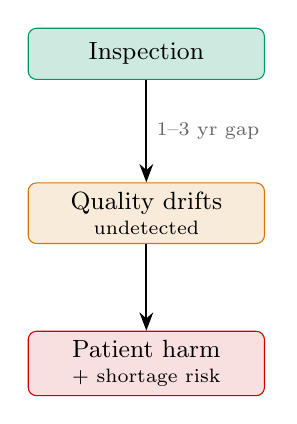
\begin{tikzpicture}[
  box/.style={rectangle, rounded corners=3pt, draw, minimum width=3.0cm,
              minimum height=0.65cm, font=\small, align=center},
  arr/.style={-{Stealth}, thick}
]
\node[box, fill=govGreen!20, draw=govGreen] (insp) {Inspection};
\node[box, fill=warnOrange!15, draw=warnOrange, below=1.3cm of insp] (drift)
  {Quality drifts\\[-2pt]{\scriptsize undetected}};
\node[box, fill=ncsuRed!12, draw=ncsuRed, below=1.1cm of drift] (harm)
  {Patient harm\\[-2pt]{\scriptsize + shortage risk}};
\draw[arr] (insp) -- node[right, font=\scriptsize, text=ncsuGray] {1--3 yr gap} (drift);
\draw[arr] (drift) -- (harm);
\end{tikzpicture}
\end{columns}
\end{frame}

\begin{frame}{FDA Form 483: Structure and the Classification Gap}
\begin{columns}[T]
\column{0.40\textwidth}

{\small
\textbf{483} issued at close -- inspector-written deficiency list\\[5pt]
\textbf{EIR} written after -- full narrative, exhibits, responses\\[5pt]
\textbf{Classification} assigned later:\\[4pt]
\quad \textcolor{govGreen}{\textbf{NAI}} ~\textcolor{ncsuGray}{\small No Action}\\
\quad \textcolor{warnOrange}{\textbf{VAI}} ~\textcolor{ncsuGray}{\small Voluntary Action}\\
\quad \textcolor{ncsuRed}{\textbf{OAI}} ~\textcolor{ncsuGray}{\small Official Action}
}

\vspace{8pt}
\begin{itemize}
  \setlength{\itemsep}{6pt}
  \item<2-> We have \textbf{483 text} (FOIA via Redica) -- EIR inaccessible
  \item<3-> Three outcome labels \textbf{discard} most inspection content -- 483 text carries what the label cannot
\end{itemize}

\column{0.57\textwidth}
\begin{center}
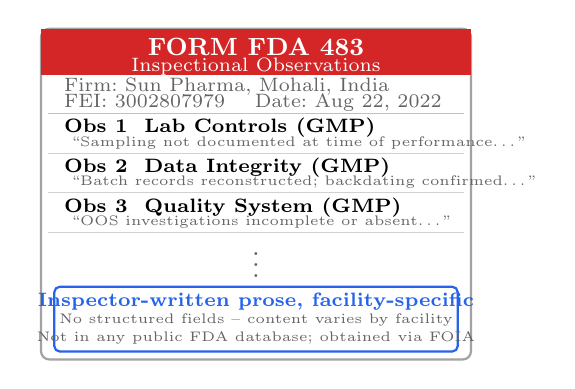
\begin{tikzpicture}[scale=0.84]
\draw[rounded corners=3pt, thick, draw=ncsuGray!60, fill=white]
  (0,0) rectangle (6.5,5.0);
\fill[ncsuRed!85] (0,4.3) rectangle (6.5,5.0);
\node[white, font=\small\bfseries] at (3.25,4.72) {FORM FDA 483};
\node[white, font=\scriptsize] at (3.25,4.43) {Inspectional Observations};
\node[right, font=\scriptsize, text=ncsuGray] at (0.2,4.12)
  {Firm:~Sun Pharma, Mohali, India};
\node[right, font=\scriptsize, text=ncsuGray] at (0.2,3.88)
  {FEI:~3002807979 \quad Date:~Aug 22, 2022};
\draw[ncsuGray!40] (0.1,3.72) -- (6.4,3.72);
\node[right, font=\scriptsize\bfseries] at (0.2,3.50)
  {Obs 1~~Lab Controls (GMP)};
\node[right, font=\tiny, text=ncsuGray] at (0.3,3.28)
  {``Sampling not documented at time of performance\ldots''};
\draw[ncsuGray!30] (0.1,3.12) -- (6.4,3.12);
\node[right, font=\scriptsize\bfseries] at (0.2,2.90)
  {Obs 2~~Data Integrity (GMP)};
\node[right, font=\tiny, text=ncsuGray] at (0.3,2.68)
  {``Batch records reconstructed; backdating confirmed\ldots''};
\draw[ncsuGray!30] (0.1,2.52) -- (6.4,2.52);
\node[right, font=\scriptsize\bfseries] at (0.2,2.30)
  {Obs 3~~Quality System (GMP)};
\node[right, font=\tiny, text=ncsuGray] at (0.3,2.08)
  {``OOS investigations incomplete or absent\ldots''};
\draw[ncsuGray!30] (0.1,1.92) -- (6.4,1.92);
\node[font=\normalsize, text=ncsuGray] at (3.25,1.55) {\vdots};
\draw[techBlue, rounded corners=2pt, thick] (0.2,0.12) rectangle (6.3,1.1);
\node[font=\scriptsize\bfseries, text=techBlue] at (3.25,0.88)
  {Inspector-written prose, facility-specific};
\node[font=\tiny, text=ncsuGray] at (3.25,0.60)
  {No structured fields -- content varies by facility};
\node[font=\tiny, text=ncsuGray] at (3.25,0.32)
  {Not in any public FDA database; obtained via FOIA};
\end{tikzpicture}
\end{center}

\vspace{4pt}
\onslide<4->{
\begin{alertblock}{Research question}
\small Do 483 text signals predict patient harm and differentiate facilities with the same outcome label?
\end{alertblock}
}
\end{columns}
\end{frame}

% ── SECTION 2: STUDY DESIGN ──────────────────────────────────────────────────
\section{Study Design \& Data}

\begin{frame}{Study Design: 14 Drugs, 98 Facilities, 2018–2026}

\onslide<1->{
\textbf{Drug and facility universe:}
\begin{itemize}
  \item \highlight{14 generic APIs} spanning cardiovascular, anti-infective, and critical care classes
  \item 129 FEIs identified via NDC $\to$ DailyMed label $\to$ facility crosswalk
\end{itemize}
}

\vspace{5pt}
\onslide<2->{
\textbf{Inspection text and outcomes (Redica):}
\begin{itemize}
  \item \highlight{98 FEIs} with Form 483 text and NAI/VAI/OAI classifications
  \item \highlight{246 inspection events}, 2018--2026
\end{itemize}
}

\vspace{5pt}
\onslide<3->{
\textbf{Outcome variable: serious adverse events (FAERS):}
\begin{itemize}
  \item FAERS reports carry an ANDA number -- linked to producing facility via Orange Book
  \item Serious outcomes only: death, hospitalization, disability
  \item \highlight{78 of 98 FEIs} have ANDA-matched AE data; 20 have no FAERS reports citing their ANDA
\end{itemize}
}

\vspace{5pt}
\onslide<4->{
\textbf{Panel:} one row per inspection, $\pm$4 quarters. \highlight{246 rows} total (text features); \highlight{176 rows} with ANDA-matched outcome.
}

\end{frame}

% ── SECTION 3: LLM PIPELINE ──────────────────────────────────────────────────
\section{LLM Extraction Pipeline}

\begin{frame}{Pipeline: From 483 Text to Structured Features}

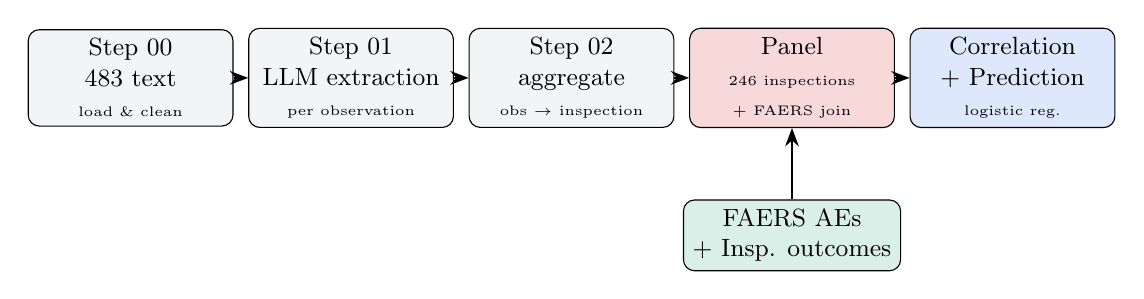
\begin{tikzpicture}[
  box/.style={rectangle, rounded corners=4pt, draw, fill=lightGray,
              minimum height=0.7cm, minimum width=2.6cm, font=\small, align=center},
  arrow/.style={-{Stealth}, thick}
]
% Step 0
\node[box] (s0) at (0,0) {Step 00\\483 text\\{\tiny load \& clean}};
% Step 1
\node[box] (s1) at (2.8,0) {Step 01\\LLM extraction\\{\tiny per observation}};
% Step 2
\node[box] (s2) at (5.6,0) {Step 02\\aggregate\\{\tiny obs $\to$ inspection}};
% Panel
\node[box, fill=ncsuRed!15] (panel) at (8.4,0) {Panel\\{\tiny 246 inspections}\\{\tiny + FAERS join}};
% Model
\node[box, fill=techBlue!15] (model) at (11.2,0) {Correlation\\+ Prediction\\{\tiny logistic reg.}};

\draw[arrow] (s0) -- (s1);
\draw[arrow] (s1) -- (s2);
\draw[arrow] (s2) -- (panel);
\draw[arrow] (panel) -- (model);

% Data joins below panel
\node[box, fill=govGreen!15] (faers) at (8.4,-2.0) {FAERS AEs\\+ Insp. outcomes};
\draw[arrow] (faers) -- (panel);

\end{tikzpicture}

\end{frame}

% ── SECTION 4: LLM EXTRACTION ────────────────────────────────────────────────
\section{LLM Extraction Pipeline}

\begin{frame}{Step 00: What a 483 Observation Looks Like in Practice}
{\small \textbf{Sun Pharma, Mohali -- Aug 2022 OAI inspection.} 6 observations. Two shown below.}

\vspace{5pt}
\begin{columns}[T]
\column{0.48\textwidth}
\onslide<1->{
\begin{block}{Observation 1 \hfill \textcolor{warnOrange}{\scriptsize Data Integrity}}
\scriptsize
\textbf{Header:} ``There is a failure to thoroughly review any unexplained discrepancy whether or not the batch has been already distributed.''

\vspace{4pt}
\textbf{Sub-item:} ``Disclosure 2020-01 confirmed instances of backdating by QA and QC personnel. The investigation was not thorough to evaluate the scope of backdating in the QA and QC departments.''

\vspace{3pt}
\textit{[3 sub-items with nested detail -- 2 pages]}
\end{block}
}

\column{0.48\textwidth}
\onslide<2->{
\begin{block}{Observation 2 \hfill \textcolor{techBlue}{\scriptsize Lab Controls}}
\scriptsize
\textbf{Header:} ``Established sampling plans, test procedures and laboratory control mechanisms are not documented at the time of performance.''

\vspace{4pt}
\textbf{Sub-item:} ``Building access records showed an employee responsible for collecting samples did not enter the buildings where samples were documented to have been collected.''

\vspace{3pt}
\textit{[2 sub-items with dated examples -- 1.5 pages]}
\end{block}
}
\end{columns}

\vspace{6pt}
{\small
\begin{itemize}
  \setlength{\itemsep}{3pt}
  \item<3-> One inspection, two domains, two different risk profiles
  \item<4-> Risk signals embedded in prose -- no structured fields
  \item<5-> Facility-specific: mean Jaccard\,=\,0.10 across 1,067 observations
\end{itemize}
}
\end{frame}

\begin{frame}{Step 01: What the LLM Extracts}
\begin{columns}[T]
\column{0.50\textwidth}
\textbf{Group 1: Binary flags} {\footnotesize (True/False per observation)}

\vspace{3pt}
{\small
\begin{itemize}
  \setlength{\itemsep}{4pt}
  \item \textbf{Data integrity (DI)} -- falsification, backdating, reconstructed records
  \item \textbf{Contamination} -- microbial, chemical, or cross-product
  \item \textbf{Patient risk} -- direct patient harm pathway
  \item \textbf{Investigation failure} -- OOS investigation absent or inadequate
  \item \textbf{Repeat finding} -- same citation at a prior inspection
\end{itemize}
}

\column{0.47\textwidth}
\pause
\textbf{Group 2: Multi-category signals}

\vspace{3pt}
{\small
\begin{itemize}
  \setlength{\itemsep}{4pt}
  \item \textbf{Domain} -- 8 CFR\,211 areas (Lab Controls, Quality System\ldots)
  \item \textbf{Severity} -- Critical / Major / Moderate / Minor
  \item \textbf{Root cause} -- Capital (resource gap) vs.\ Cultural (management gap)
  \item \textbf{Scope} -- SingleBatch / MultipleProducts / FacilityWide
  \item \textbf{Remediation} -- corrective action language present or absent
\end{itemize}
}
\end{columns}
\end{frame}

\begin{frame}{Step 01: Turning Unstructured Inspection Text into Structured Features}
\begin{columns}[T]
\column{0.58\textwidth}
\begin{block}{Input: verbatim 483 observation text}
\scriptsize
``Batch production records were not completed at the time of manufacture. Entries were reconstructed from memory 2 days after processing.''
\end{block}

\vspace{4pt}
\textbf{Output (Claude Haiku, one pass per observation):}

\vspace{2pt}
{\scriptsize
\begin{tabular}{lll}
\toprule
Dimension & Extracted value & Rationale \\
\midrule
Severity & \textbf{Major} & confirmed defect; records reconstructed \\
DI flag  & \textbf{True}  & reconstructed entries = DI trigger \\
\bottomrule
\end{tabular}
}

\vspace{8pt}
{\small
\begin{itemize}
  \setlength{\itemsep}{5pt}
  \item Fixed JSON schema -- model cannot invent fields
  \item Future work: multi-LLM benchmark + Redica human-in-loop verification
\end{itemize}
}

\column{0.39\textwidth}
\textbf{How trustworthy is the extraction?}

\vspace{5pt}
\begin{itemize}
  \setlength{\itemsep}{5pt}
  \item Claude 3.0 Haiku: 90.2\% on clinical entity extraction (Khairallah et al., 2024)
  \item Prompt definitions reviewed by Redica GMP specialists (June 2026)
  \item Human validation in progress; treat findings as preliminary
\end{itemize}
\end{columns}
\end{frame}

\begin{frame}{Step 02: From Observation Labels to Inspection Feature Vectors}
\begin{columns}[T]
\column{0.52\textwidth}
\textbf{Three types of features per inspection:}

\vspace{6pt}
\textbf{1. Share} -- fraction of observations in a domain or with a flag\\
{\small\textit{e.g.} \texttt{vc\_labcontrols\_share}: what kind of inspection was this?}

\pause
\vspace{6pt}
\textbf{2. Count} -- raw number of observations in a domain\\
{\small\textit{e.g.} \texttt{n\_labcontrols\_obs}: how much was cited?}

\pause
\vspace{6pt}
\textbf{3. Co-occurrence} -- both signals present in the same inspection\\
{\small\textit{e.g.} \texttt{joint\_labctrl\_di}: Lab Controls \emph{and} DI in one visit}

\column{0.45\textwidth}
\textbf{Why co-occurrence matters:}

\vspace{6pt}
{\small
Lab Controls alone: QC process failed.\\[4pt]
DI alone: record altered.\\[4pt]
\textbf{Both together:} stronger combined signal than either alone.
}

\vspace{10pt}
\begin{block}{Output}
\small 246 inspections $\times$ 17 features
\end{block}
\end{columns}
\end{frame}

% ── SECTION 5: THEORY ────────────────────────────────────────────────────────
\section{Analysis}

\begin{frame}{Do 483 Text Signals Carry Information? Evidence From the VAI-Only Subgroup}
\begin{columns}[T]
\column{0.50\textwidth}
\textbf{AUC, 5-fold FEI-grouped CV (176 inspections, 78 FEIs with ANDA-matched AEs):}

\vspace{4pt}
{\small
\begin{tabular}{clcc}
\toprule
 & Feature set & LR AUC & \\
\midrule
A & Text only (17 LLM features) & 0.585 & \\
B & Text + inspection outcome flag & 0.583 & \\
C & Inspection outcome flag only & 0.545 & \\
\midrule
\multicolumn{2}{l}{\textit{Random baseline}} & \textit{0.500} & \\
\midrule
\pause
\highlight{D} & \highlight{Text only, VAI-only facilities} & \highlight{0.656} & $p{=}0.046$ \\
E & Text only, OAI-ever facilities & 0.473 & \\
\bottomrule
\multicolumn{4}{l}{\scriptsize $p$ from one-tailed $t$-test vs.\ 0.5 across 5 CV folds}
\end{tabular}
}

\vspace{4pt}
{\small Config D: 55 VAI-only FEIs, 110 inspections.}

\hfill\column{0.42\textwidth}
\begin{itemize}
  \setlength{\itemsep}{7pt}
  \item \textbf{Full sample (A--C):} text (0.585) beats the OAI flag (0.545); combining adds no gain
  \pause
  \item \textbf{VAI-only (D):} \highlight{AUC\,=\,0.66} ($p{=}0.046$) -- text separates facilities where the outcome label cannot
  \pause
  \item \textbf{OAI-ever (E):} text adds little -- enforcement likely corrected the problems
\end{itemize}
\end{columns}
\end{frame}

% ── SECTION 8: TRAJECTORY ANALYSIS ──────────────────────────────────────────
\section{Trajectory Analysis}

\begin{frame}{The Silent Problem: Same VAI Label, Very Different Patient Outcomes}
\begin{columns}[T]
\column{0.52\textwidth}
{\small \textbf{AEs by facility group} (98 FEIs, FEI-level medians):}

\vspace{4pt}
{\scriptsize
\begin{tabular}{lccc}
\toprule
Group & $n$ & Q0 & Q+4 \\
\midrule
OAI-ever & 25 & 32 & 30 \\
\rowcolor{techBlue!12}
Hi-sig VAI & 19 & 40 & \highlight{49} \\
Lo-sig VAI & 54 & 34 & 30 \\
\bottomrule
\end{tabular}
}

\vspace{14pt}
\pause
{\small \textbf{Top Lab Controls facilities (VAI-only), by AE rise:}}

\vspace{4pt}
{\scriptsize
\begin{tabular}{lccc}
\toprule
Manufacturer / Drug & Q0 & Q+4 & Rise \\
\midrule
Lupin / Atorvastatin      & 31 & \highlight{44} & \highlight{$+$42\%} \\
Dr.\ Reddy's / Metoprolol & 80 & \highlight{97} & \highlight{$+$21\%} \\
Sun / Atorvastatin        & 80 & \highlight{87} & \highlight{$+$9\%}  \\
\bottomrule
\end{tabular}
}

\vspace{3pt}
{\scriptsize AEs per quarter (manufacturer-specific). Hi-sig VAI = top-quartile Lab Controls share, never OAI.}

\column{0.45\textwidth}
\begin{itemize}
  \setlength{\itemsep}{9pt}
  \item \textbf{63\% more AEs at Q+4} (49 vs.\ 30), same FDA label -- named examples show persistent rise with no OAI
  \pause
  \item \textbf{OAI$\to$VAI downgrade} documented (ProPublica, Bloomberg): reclassified under shortage pressure; downgraded facilities show worse outcomes
  \pause
  \item Alternatively: findings stayed below OAI threshold or severity was not surfaced
\end{itemize}
\end{columns}
\end{frame}

% ── SECTION 10: SUMMARY ──────────────────────────────────────────────────────
\section{Summary}

\begin{frame}{Summary}

\begin{enumerate}
  \setlength{\itemsep}{8pt}
  \item \textbf{Yes -- 483 text is associated with future harm, but primarily among facilities FDA never penalized.}\\
    VAI-only AUC = \highlight{0.656}; in the full sample, text (0.585) modestly outperforms the inspection outcome flag (0.545).
  \pause

  \item \textbf{Same VAI label, very different outcomes -- and identifiable from text.}\\
    Hi-sig VAI facilities produce 63\% more AEs at Q+4 than Lo-sig VAI (49 vs.\ 30). These facilities can be ranked from 483 text alone; shortage pressure may explain why enforcement did not follow.
\end{enumerate}

\end{frame}

% ── SECTION 11: LIMITATIONS & NEXT STEPS ─────────────────────────────────────
\section{Limitations \& Next Steps}

\begin{frame}{Limitations}
\begin{columns}[T]
\column{0.50\textwidth}
\begin{itemize}
  \setlength{\itemsep}{6pt}
  \item \textbf{Sample size:} 98 FEIs, 33 OAI. VAI-only results are hypothesis-generating.
  \item \textbf{COVID gap:} inspections suspended 2020--21; post-2022 baselines are confounded.
  \item \textbf{FAERS attribution:} multi-facility ANDAs cannot be linked to a specific site.
\end{itemize}

\pause
\column{0.47\textwidth}
\begin{itemize}
  \setlength{\itemsep}{6pt}
  \item \textbf{Extraction quality:} human validation in progress; treat as preliminary.
  \item \textbf{Volume:} commercial volume not integrated; size is a confounder.
  \item \textbf{Causal:} all associations are correlational; shortage-pressure hypothesis requires market data.
\end{itemize}
\end{columns}
\end{frame}

% ── Q&A SLIDE ─────────────────────────────────────────────────────────────────

\begin{frame}{}
\begin{center}
\vspace{2.2cm}
{\Large \textbf{Questions \& Discussion}}\\[20pt]
{\normalsize \texttt{asahebi@ncsu.edu}}
\end{center}
\end{frame}

\end{document}
